% vim: set fenc=utf-8 ft=latex encoding=utf-8
% -*- mode: latex; coding: UTF-8; -*-

\newif\ifdraft
\drafttrue

%%% Marching Triangles.tex

%%%
%%% - ``review'' for content submitted for review
%%% - ``preprint'' for accepted content making available.
%%% - ``tog'' for technical papers accepted to the TOG journal and
%%%	for presentation at the SIGGRAPH or SIGGRAPH Asia conference.
%%% - ``conference'' for final content accepted to a sponsored event
%%% 	(hint: if unsure, use ``conference'') %%% \documentclass[review]{acmsiggraph}

\ifdraft
	\documentclass[conference]{acmsiggraph}
	\def\baselinestrech{1}
	\setlength{\marginparwidth}{2cm}
	\newcommand{\Title}{Investigating Toplogies of Marching Triangles | DRAFT}
\else
	\documentclass[conference]{acmsiggraph}
	\newcommand{\Title}{Investigating Toplogies of Marching Triangles}
\fi


\newcommand{\Author}{Evan T. C. Wilde}
\newcommand{\Email}{etcwilde@uvic.ca}
\newcommand{\Subject}{Using marching triangles algorithm on implicit surfaces}
\newcommand{\Keywords}{iso-surface, polygonization, marching-triangles}

\synctex=1

\usepackage{xspace}

%% \usepackage[unicode=true,
%% 	bookmarks=false,breaklinks=flase,pdfborder={0 0 0},
%% 	backref=none,colorlinks=false]{hyperref}

\hypersetup{pdftitle={\Title},
	pdfauthor={\Author},
	pdfkeywords={\Keywords},
	pdfsubject={\Subject},
	urlcolor=blue,citecolor=cyan}

\def\BibTeX{{\rm B\kern-.05em{\sc i\kern-.025em b}\kern-.08em
    T\kern-.1667em\lower.7ex\hbox{E}\kern-.125emX}}

\TOGonlineid{V00775033}
\TOGvolume{0}
\TOGnumber{0}

\ifdraft
	\usepackage[colorinlistoftodos]{todonotes}
		\newcommand{\evan}[1]{{\color{cyan}\emph{Evan Says:
		#1}}\xspace}
		\newcommand{\evanTodo}[1]{{\color{blue}\emph{Evan Todo:
		#1}}\xspace}
\else
	\usepackage[disable]{todonotes}
	\newcommand{\evan}[1]{}
	\newcommand{\evanTodo}[1]{}
\fi

\newcommand{\fff}{field falloff function}


%%% Local Variables:
%%% mode: latex
%%% TeX-master: "marching-triangles"
%%% End:


\title{\Title}
\author{
	\Author \\
	University of Victoria\\
	\Email}
\pdfauthor{\Author}
\keywords{\Keywords}

\begin{document}
%%% This is the ``teaser'' command, which puts an figure, centered, below
%%% the title and author information, and above the body of the content.

\teaser{
	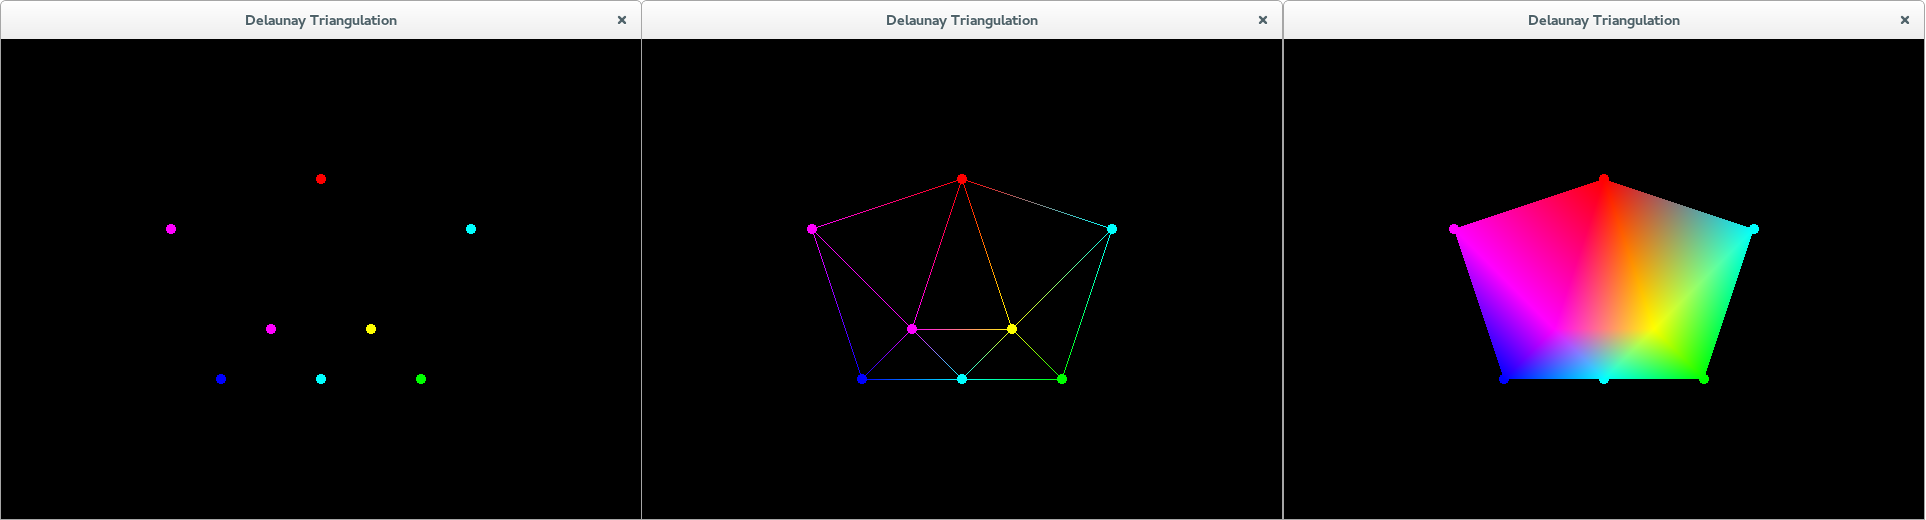
\includegraphics[height=1.5in] {images/Heading.png}
	\caption{Delaunay Triangulation}
}

\maketitle

\begin{abstract}
	In this paper, I describe a method of implementing the marching
	triangles algorithm to polygonize implicit surfaces. The marching
	triangles algorithm provides a technique of generating optimal
	triangulations of a surface, while eliminating ambiguous cases found in
	other polygonization algorithms. The marching triangle algorithm, also
	known as the advancing front algorithm, grows the mesh from a seed
	triangle, until the surface is covered. This growth of single triangles
	allows the algorithm to generate a mesh that more closely represents
	the topology of the surface while minimizing polygons.
\end{abstract}

\keywordlist

\copyrightspace

\section{Introduction}
Implicit surfaces (iso-surfaces) provide a method to store complex geometry or
geometry that cannot be generated in an explicit manner. An iso-surface is
specified with a mathematical formula, and can specify arbitrary geometry. It
is useful in physical simulations and in the games industries. An iso-surface
can contain a massive amount of information, while not requiring as much space.

While iso-surfaces contain lots of detail accurately, computers have difficulty
representing them visually. There are two methods for creating a visual
representation of an iso-surface: raytracing or a polygonization algorithm.

Raytracing the surface produces the most accurate visual representation, the
accuracy is only limited by the dimensions of the image being generated, at the
cost of speed. Even with state-of-the-art hardware and the most optimized
raytacing algorithms, raytracers are unable to produce images quickly enough
for interactive real-time rendering of implicit surfaces.

Currently, a very popular polygonization algorithm is the Marching Cubes, which
fills the universe with voxels, determines how the surface intersects each
voxel, and results in a plane within the voxel. This results in triangles which
are non-optimal to the topology of the surface, furthermore, there are
ambiguous cases where geometry is lost or cracks emerge.

An ideal polygonization would meet the following criteria:
it would produce a mesh that does not distort triangles, that is there are no
triangles that are long and narrow; it would produce triangles small enough
that no features of the surface are lost; smooth, flat, surfaces would not be
broken into more triangles than necessary; the mesh should not have holes or
disconnected vertices.

The Marching Triangles (MT) algorithm has the potential to create such a
polygonization. The marching triangles is an incremental algorithm that uses
the curvature of the surface to determine where new vertices are placed, either
creating larger triangles where the curvature is small, or creating smaller
triangles where the curvature is large.

In this paper, I investigate the range of geometric topologies the Marching
Triangles algorithm is capable of successfully polygonizing.

\section{Related Work}

Research has been performed on converting point-cloud data to triangulations
using a form of the marching triangles algorithm\cite{Scheidegger2005}. This
area is helpful for visualizing the data collected from different sensors
such as, ultrasound pings for robots, LIDAR scans for ocean bathymetry, 3D
scans of objects, or any application where discrete vertices in 3-dimensional
space must be converted to a continuous mesh. The method, also known as the
``Advancing Front algorithm'' builds triangulations of the point cloud using a
3-dimensional generalization of Delaunay triangulation to create a mesh
representation where the triangles are not distorted.

Akkouche presents an implementation of the marching triangles algorithm for
closed implicit surface manifolds\cite{Akkouche2001}. The algorithm provided
topologically correct and geometrically accurate triangle meshes for closed
surfaces. Their results suggest that the marching triangles algorithm runs in
comparable time to the marching cubes algorithm, though the resulting mesh has
higher visual appeal and better overall quality due to the adaptive triangle
size.

\section{Marching Triangles Algorithm}
The marching triangles algorithm creates a seed triangle and adds the three
edges to an edge pool. Then it selects one of the edges at random then
generates a new vertex in the direction of the gradient. If the curvature is
too great, the vertex will be brought closer to the selected edge, otherwise it
will push the vertex away. Once the vertex is placed, two new edges are added
between the vertices of the selected edge and the new vertex to generate a new
triangle. Then the selected edge is removed from the edge pool. The process of
selecting an edge and new vertex continues until the surface is covered.

\section {Implementation}

\subsection{Delaunay Triangulation}
I began with an implementation of the Delaunay triangulation to look at
possible methods of triangulation. Because the triangulation runs on a
point-cloud it won't be useful in the generation of triangles in the mesh. It
may be useful to create a circumsphere that bounds the size of the triangle so
that a triangle will never be too long in relation to the width.
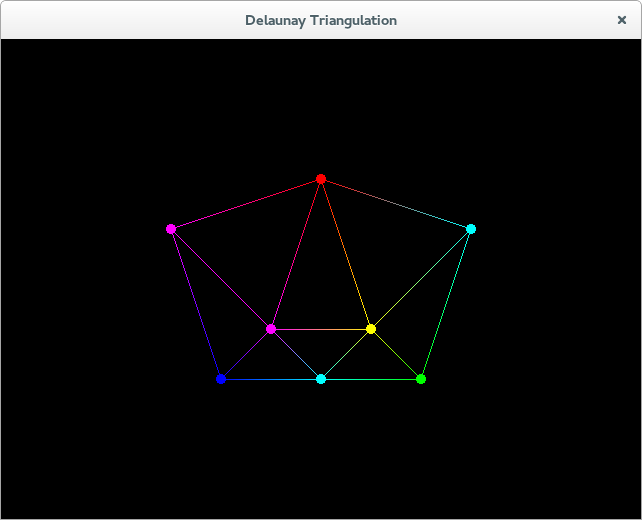
\includegraphics[height=1.5in]{images/Triangulated.png}

\section{Results}
No results yet\ldots.

\evanTodo{Find results!}

\section{Conclusion}
No conclusive information yet\ldots.

\evanTodo{Make conclusions}

\bibliographystyle{acmsiggraph}
\bibliography{references}



\end{document}

